\documentclass[journal,12pt,twocolumn]{IEEEtran}
%

\usepackage{setspace}
\usepackage{gensymb}
\singlespacing

\usepackage{amsmath}
\usepackage{amsthm}
\usepackage{txfonts}
\usepackage{cite}
\usepackage{enumitem}
\usepackage{mathtools}
\usepackage{listings}
    \usepackage{color}                                            %%
    \usepackage{array}                                            %%
    \usepackage{longtable}                                        %%
    \usepackage{calc}                                             %%
    \usepackage{multirow}                                         %%
    \usepackage{hhline}                                           %%
    \usepackage{ifthen}                                           %%
  %optionally (for landscape tables embedded in another document): %%
    \usepackage{lscape}     
\usepackage{multicol}
\usepackage{chngcntr}
\usepackage{tikz}
\usepackage{pgfplots}
\renewcommand\thesection{\arabic{section}}
\renewcommand\thesubsection{\thesection.\arabic{subsection}}
\renewcommand\thesubsubsection{\thesubsection.\arabic{subsubsection}}

\renewcommand\thesectiondis{\arabic{section}}
\renewcommand\thesubsectiondis{\thesectiondis.\arabic{subsection}}
\renewcommand\thesubsubsectiondis{\thesubsectiondis.\arabic{subsubsection}}

% correct bad hyphenation here
\hyphenation{op-tical net-works semi-conduc-tor}
\def\inputGnumericTable{}                                 %%

\lstset{
%language=C,
frame=single, 
breaklines=true,
columns=fullflexible
}

\begin{document}
%


\newtheorem{theorem}{Theorem}[section]
\newtheorem{problem}{Problem}
\newtheorem{proposition}{Proposition}[section]
\newtheorem{lemma}{Lemma}[section]
\newtheorem{corollary}[theorem]{Corollary}
\newtheorem{example}{Example}[section]
\newtheorem{definition}[problem]{Definition}
\newcommand{\BEQA}{\begin{eqnarray}}
\newcommand{\EEQA}{\end{eqnarray}}
\newcommand{\define}{\stackrel{\triangle}{=}}
\bibliographystyle{IEEEtran}
\providecommand{\mbf}{\mathbf}
\providecommand{\pr}[1]{\ensuremath{\Pr\left(#1\right)}}
\providecommand{\qfunc}[1]{\ensuremath{Q\left(#1\right)}}
\providecommand{\sbrak}[1]{\ensuremath{{}\left[#1\right]}}
\providecommand{\lsbrak}[1]{\ensuremath{{}\left[#1\right.}}
\providecommand{\rsbrak}[1]{\ensuremath{{}\left.#1\right]}}
\providecommand{\brak}[1]{\ensuremath{\left(#1\right)}}
\providecommand{\lbrak}[1]{\ensuremath{\left(#1\right.}}
\providecommand{\rbrak}[1]{\ensuremath{\left.#1\right)}}
\providecommand{\cbrak}[1]{\ensuremath{\left\{#1\right\}}}
\providecommand{\lcbrak}[1]{\ensuremath{\left\{#1\right.}}
\providecommand{\rcbrak}[1]{\ensuremath{\left.#1\right\}}}
\theoremstyle{remark}
\newtheorem{rem}{Remark}
\newcommand{\sgn}{\mathop{\mathrm{sgn}}}
\providecommand{\abs}[1]{\left\vert#1\right\vert}
\providecommand{\res}[1]{\Res\displaylimits_{#1}} 
\providecommand{\norm}[1]{\left\lVert#1\right\rVert}
\providecommand{\mtx}[1]{\mathbf{#1}}
\providecommand{\mean}[1]{E\left[ #1 \right]}
\providecommand{\fourier}{\overset{\mathcal{F}}{ \rightleftharpoons}}
\providecommand{\system}{\overset{\mathcal{H}}{ \longleftrightarrow}}
\newcommand{\solution}{\noindent \textbf{Solution: }}
\newcommand{\cosec}{\,\text{cosec}\,}
\providecommand{\dec}[2]{\ensuremath{\overset{#1}{\underset{#2}{\gtrless}}}}
\newcommand{\myvec}[1]{\ensuremath{\begin{pmatrix}#1\end{pmatrix}}}
\newcommand{\cmyvec}[1]{\ensuremath{\begin{pmatrix*}[c]#1\end{pmatrix*}}}
\newcommand{\mydet}[1]{\ensuremath{\begin{vmatrix}#1\end{vmatrix}}}
\newcommand{\proj}[2]{\textbf{proj}_{\vec{#1}}\vec{#2}}
\let\StandardTheFigure\thefigure
\let\vec\mathbf
\title{Assignment - 2}
\author{Arjun Jayachandran
\\ MD/2020/702}
% make the title area
\maketitle
\newpage
%\tableofcontents
\bigskip
\renewcommand{\thefigure}{\theenumi}
\renewcommand{\thetable}{\theenumi}
%\renewcommand{\theequation}{\theenumi}
\begin{abstract}
This is a simple document to learn about vectors and matrices and present it using latex, draw figures using Python, Latex.
\end{abstract}
%Download all python codes 
%
%\begin{lstlisting}
%svn co https://github.com/JayatiD93/trunk/My_solution_design/codes
%\end{lstlisting}
Download all and latex-tikz codes from 
%
\begin{lstlisting}
svn co https://github.com/arjunjc93/Assignment-2.git
\end{lstlisting}
%
\section{Vectors\\(Points and Vectors by G V V Sharma Exercises-Q.2.10)}
\renewcommand{\theequation}{\theenumi}
\begin{enumerate}[label=\thesection.\arabic*.,ref=\thesection.\theenumi]
\numberwithin{equation}{enumi}
\item In each of the following, find the value of \emph{k} for which the points are collinear
\begin{enumerate}
    \item \myvec{7\\-2}, \myvec{5\\1}, \myvec{3\\\emph{k}}
    \item \myvec{8\\1}, \myvec{\emph{k}\\-4}, \myvec{2\\-5}
\end{enumerate}
\solution\begin{enumerate}
    \item Let
    \begin{align}
        \vec{A}=\myvec{7\\-2}, \vec{B}=\myvec{5\\1}, \vec{C}=\myvec{3\\k}
    \end{align}\\
    Then,
    \begin{align}
        \vec{B}-\vec{A}=\myvec{-2\\3}, \vec{C}-\vec{A}=\myvec{-4\\\emph{k}+2}
    \end{align}
    and
    \begin{align}
     \vec{M}=\myvec{\vec{B}-\vec{A}&\vec{C}-\vec{A}}^T\end{align}
     \begin{align}
         =\myvec{-2 & 3\\-4 & \emph{k}+2} \xleftrightarrow{R_2 \leftarrow 2R_1-R_2}
     \myvec{-2&3\\0&4-\emph{k}}
     \end{align}
         \[\Longrightarrow \emph{rank}(\vec{M})=1 \Longleftrightarrow R_2 = \vec{0}\]
         or \[4 - \emph{k} = 0 \Longrightarrow \emph{k}=4\]
         \begin{figure}[h]
\centering
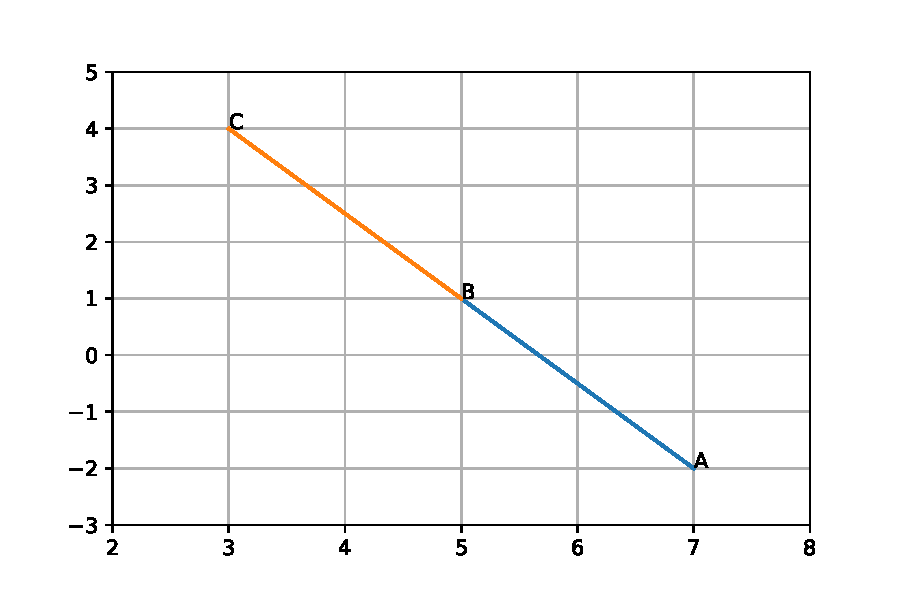
\includegraphics[width=\columnwidth]{collinear1.pdf}
\label{Fig 1.1}
\end{figure}

 \item Let
    \begin{align}
        \vec{A}=\myvec{8\\1}, \vec{B}=\myvec{\emph{k}\\-4}, \vec{C}=\myvec{2\\-5}
    \end{align}\\
    Then,
    \begin{align}
        \vec{B}-\vec{A}=\myvec{\emph{k}-8\\-5}, \vec{C}-\vec{A}=\myvec{-6\\-6}
    \end{align}
    and
    \begin{align}
     \vec{M}=\myvec{\vec{B}-\vec{A}&\vec{C}-\vec{A}}^T\end{align}
     \begin{align}
         =\myvec{\emph{k}-8 & -5\\-6 & -6} \xleftrightarrow{R_1 \leftarrow -\frac{1}{5}R_1}
     \myvec{\frac{8-\emph{k}}{5}&1\\-6&-6}\\
     \xleftrightarrow{R_2 \leftarrow 6R_1+R_2  }\myvec{\frac{8-\emph{k}}{5}& 1\\\frac{18-6\emph{k}}{5} & 0}
     \end{align}
         \[\Longrightarrow \emph{rank}(\vec{M})=1 \Longleftrightarrow R_2 = \vec{0}\]
         or \[\frac{18-6\emph{k}}{5} = 0 \Longrightarrow \emph{k}=\frac{18}{6} \Longrightarrow \emph{k}=3\]
         \begin{figure}[h]
\centering
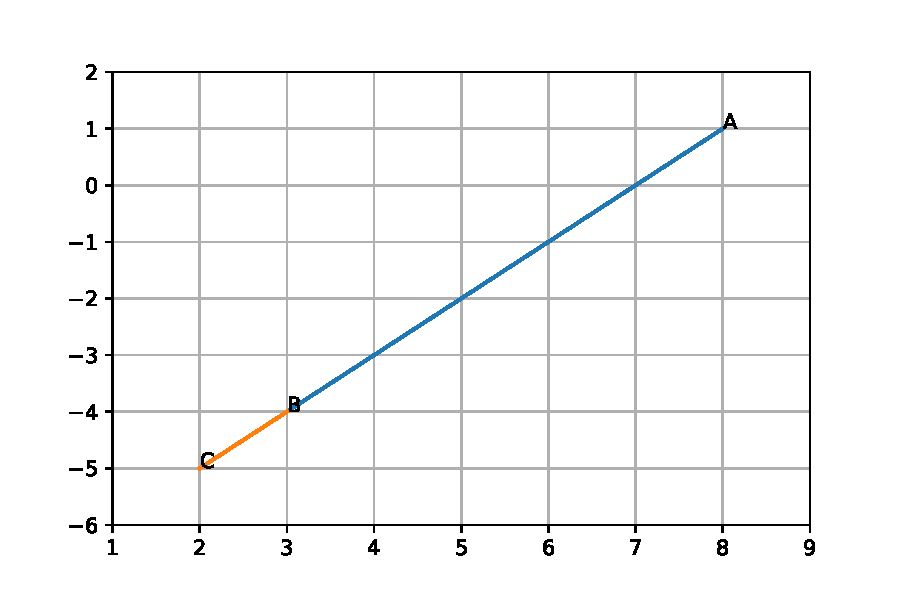
\includegraphics[width=\columnwidth]{collinear2.pdf}
\label{Fig 1.2}
\end{figure}
\end{enumerate}
\end{enumerate}
\end{document}
